

%% this section contains XX problems
%%----------------------------------------


%% Jacobs 5 steps to a 5
%%------------------------------
\element{AP}{
\begin{question}{Jacobs-Q22}
    A positive point charge enters a uniform right-ward magnetic
        field with a velocity of $v$, as diagrammed below.
    \begin{center}
        \begin{tikzpicture}
        \end{tikzpicture}
    \end{center}
    What is the direction of the magnetic force on the charge?
    \begin{choices}
        \wrongchoice{in the same direction as $v$}
        \wrongchoice{to the right}
        \wrongchoice{to the left}
        \wrongchoice{out of the page}
      \correctchoice{into the page}
    \end{choices}
\end{question}
}

\element{AP}{
\begin{question}{Jacobs-Q23}
    A long wire carries a current $I$ toward the top
        of the page.
    \begin{center}
        \begin{tikzpicture}
        \end{tikzpicture}
    \end{center}
    %% Whose left?
    What is the direction of the magnetic field produced by
        this wire to the left of the wire?
    \begin{choices}
        \wrongchoice{into the page}
      \correctchoice{out of the page}
        \wrongchoice{toward the bottom of the page}
        \wrongchoice{toward the top of the page}
      \correctchoice{to the right}
    \end{choices}
\end{question}
}

\element{AP}{
    \begin{question}{Jacobs-Q24}
    A circular loop of wire in the plane of the page
        is placed in a magnetic field pointing into
        page, as shown below.
    \begin{center}
        \begin{tikzpicture}
        \end{tikzpicture}
    \end{center}
    Which of the following will \emph{not} induce a
        current in the loop?
    \begin{choices}
      \correctchoice{moving the wire to the right in the plane of the page.}
        \wrongchoice{increasing the area of the loop}
        \wrongchoice{increasing the strength of the magnetic field}
        \wrongchoice{rotating the wire about a diameter}
        \wrongchoice{turning the magnetic field off}
    \end{choices}
\end{question}
}


%% Sample AP 2 Questions
%%------------------------------
\element{AP}{
\begin{questionmult}{AP2-Q05}
    An electron is at point $P$ in a uniform magnetic field directed into the page,
        as depicted below.
    \begin{center}
        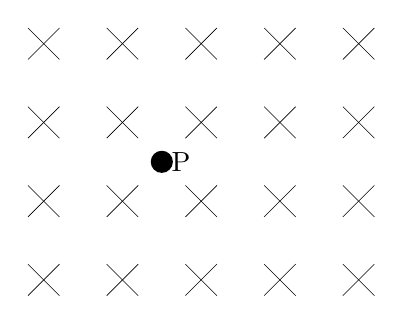
\begin{tikzpicture}[scale=2.0]
            \def\x{0.1}
            \foreach \i in {-1.0, -0.5, 0.0, 0.5, 1.0}
                \foreach \j in {-0.75, -0.25, 0.25, 0.75} {
                    \draw[very thin] (\i+\x,\j+\x) -- (\i-\x,\j-\x);
                    \draw[very thin] (\i+\x,\j-\x) -- (\i-\x,\j+\x);
                }
            \fill (-0.25,0.0) circle (2pt);
            \node[right] at (-0.25,0.0) {P};
        \end{tikzpicture}
        %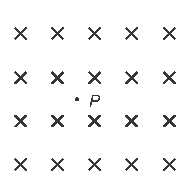
\includegraphics[keepaspectratio]{sample-AP2-Q05}
    \end{center}
    For which of the following states of motion of the electron is the magnetic
        force exerted on the electron equal to zero?
    \begin{choices}
      \correctchoice{The electron is not moving.}
      \correctchoice{The electron is moving perpendicularly into the page.}
      \correctchoice{The electron is moving perpendicularly out of the page.}
        \wrongchoice{The electron is moving.}
    \end{choices}
\end{questionmult}
}



%% 2004-APB
%%------------------------------
\element{AP}{
\begin{question}{2004-APB-Q14}
    Two parallel wires, each carrying a current $I$, repel each other
        force $F$.
    If both currents are doubled, the force of repulsion is
    \begin{choices}
        \wrongchoice{$2 F$}
        \wrongchoice{$2\sqrt{2} F$}
      \correctchoice{$4 F$}
        \wrongchoice{$4\sqrt{2} F$}
        \wrongchoice{$8 F$}
    \end{choices}
\end{question}
}

\element{AP}{
\begin{question}{2004-APB-Q47}
    Two conducting wire loops move near a very long, straight conducting
        wire that carries current $I$.
    When the loops are in the positions shown below, they are moving in
        the directions shown with the same constant speed $v$.
    \begin{center}
        %% NOTE: Add diagram
        %\includegraphics[keepaspectratio]{2004-APB-Q47}
    \end{center}
    Assume that the loops are far enough apart that they do not affect each other.
    Which of the following is true about the induced electric currents,
        if any, in the loops?
    \begin{choices}
        \wrongchoice{Loop 1: No current, Loop 2: No current}
        \wrongchoice{Loop 1: No current, Loop 2: Counterclockwise direction}
      \correctchoice{Loop 1: Clockwise direction, Loop 2: No current}
        \wrongchoice{Loop 1: Clockwise direction, Loop 2: Clockwise direction}
        \wrongchoice{Loop 1: Counterclockwise direction, Loop 2: Clockwise direction}
    \end{choices}
\end{question}
}

\element{AP}{
\begin{question}{2004-APB-Q64}
    A wire loop is rotated in a uniform magnetic field about an
        axis perpendicular to the field as shown below.
    \begin{center}
        %% NOTE: add diagram
        %\includegraphics[keepaspectratio]{2004-APB-Q64}
    \end{center}
    How many times is the induced current in the loop reversed if
        the loop makes \num{3} revolutions from the position shown?
    \begin{choices}
        \wrongchoice{One}
        \wrongchoice{Two}
        \wrongchoice{Three}
      \correctchoice{Six}
        \wrongchoice{Twelve}
    \end{choices}
\end{question}
}

